%UNIT 1: QUALITATIVE AND GRAPHICAL APPROACHES
% Is 2nd part of original 01.tex
%%%%%%%%%%%%%%%%%%%%%%%%%%%
%%%% Put the following at the top of each .tex file  %
\pagestyle{fancy}
\renewcommand{\theUnit}{1.2}
\ifthenelse{\isundefined{\UnitPageNumbers}}{}{\setcounter{page}{1}}
\rhead{Section \theUnit: Slope Fields}
\lhead{
\includegraphics[width=1.25cm]{IODE-logo.png}}
\rfoot{\mypage}
\lfoot{}
\cfoot{}
\fancypagestyle{firstfooter}{\footskip = 50pt}
\renewcommand{\footrulewidth}{.4pt}
%%%%%%%%%%%%%%%%%%%%%%%%%%%
\vspace*{-20pt} \thispagestyle{firstfooter}
\pagebegin{Slope Fields}

A \textbf{slope field} is a graphical representation of a rate of change equation. Given a rate of change equation, if we plug in particular values of $(t,y)$ then $\displaystyle\frac{dy}{dt}$ tells you the slope of the tangent vector to the solution at that point.
\vs
For example, consider the rate of change equation $\displaystyle\frac{dy}{dt}=y+2t$.  At the point (1, 3), the value of $\displaystyle\frac{dy}{dt}$ is 5. Thus, the slope field for this equation would show a vector at the point (1, 3) with slope 5.  A slope field depicts the exact slope of many such vectors, where we take each vector to be uniform length. Slope fields are useful because they provide a graphical approach for obtaining qualitatively correct graphs of the functions that satisfy a differential equation.

\begin{enumerate}
\item Below is a partially completed slope field for  $\displaystyle \frac{dP}{dt}=0.8P$. \label{01problem7}
\begin{enumerate}
\item	Plot many more tangent vectors to create a slope field. \label{01problem7parta}
\item	Use your slope field to sketch in qualitatively correct graphs of the solution functions that start at $P = 0, 0.5$, and $2$, respectively. Note: the value of $P$ at an initial time (typically $t = 0$) is called an \textbf{initial condition}. \label{01problem7partb}
\item	Recall that a solution to a differential equation is a function that satisfies the differential equation. Explain how the graph with initial condition $P(0) = 1$ can graphically be thought of as a solution to the differential equation when the differential equation is represented by its slope field. \label{01problem7partc}
\end{enumerate}

\begin{center}
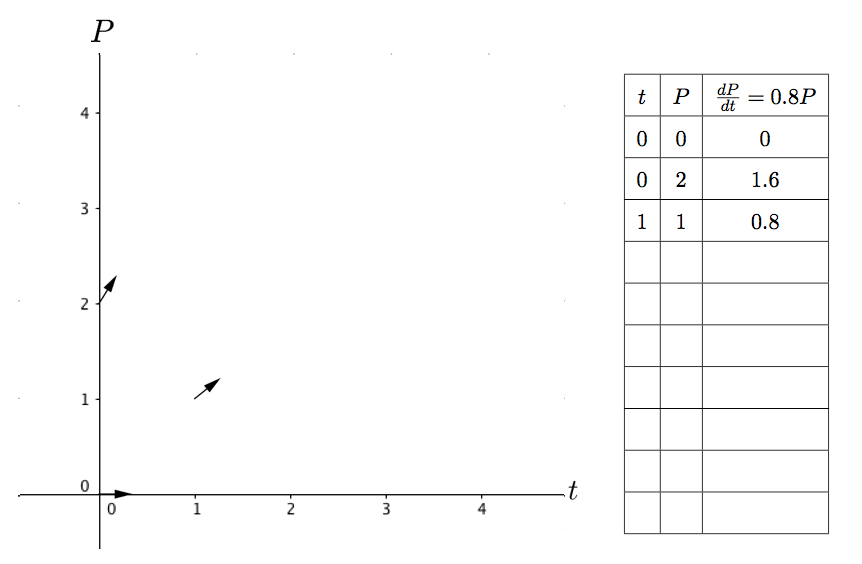
\includegraphics[width=6in]{02/02MyFirstSlopeFieldwithTable.png}
\end{center}

\clearpage

\item Below are seven rate of changes equations and three different slope fields. Without using technology, identify which differential equation is the best match for each slope field (thus you will have four rate of change equations left over). Explain your reasoning. \label{01problem8}
\[
\text{(i) } \frac{dy}{dt}=t-1 \quad \text{(ii) } \frac{dy}{dt}=1-y^2 \quad \text{(iii) } \frac{dy}{dt}=y^2-t^2 \quad \text{(iv) } \frac{dy}{dt}=1-y
\]
\[
\text{(v) } \frac{dy}{dt}=t^2-y^2 \quad \text{(vi) } \frac{dy}{dt}=1-t \quad \text{(vii) } \frac{dy}{dt}=9t^2-y^2
\]
\begin{enumerate*}
\item 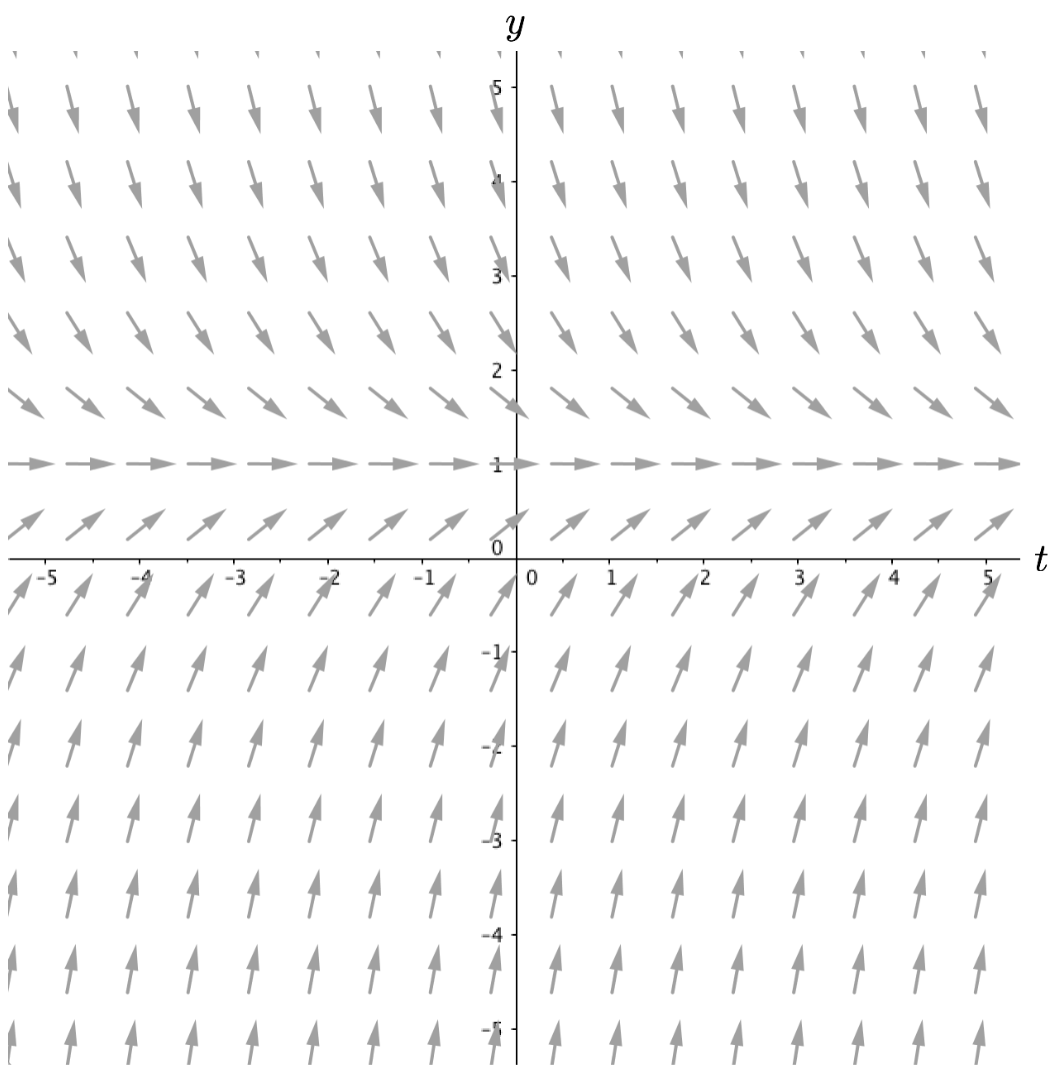
\includegraphics[width=2.75in]{02/02SlopeField1.png} \label{01problem8parta}
\item 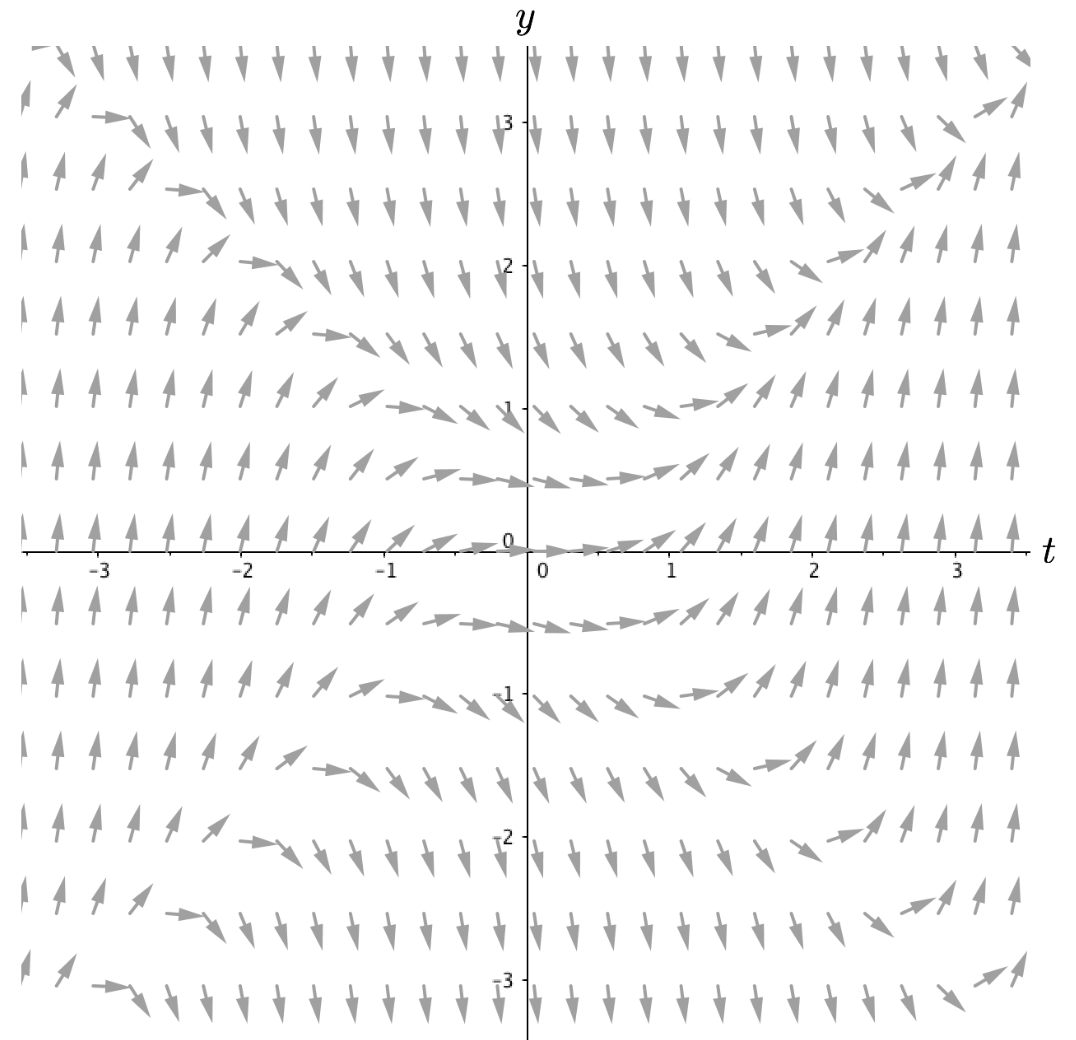
\includegraphics[width=2.75in]{02/02SlopeField2.png} \label{01problem8partb}
\end{enumerate*}

\begin{enumerate*}[resume]
\item 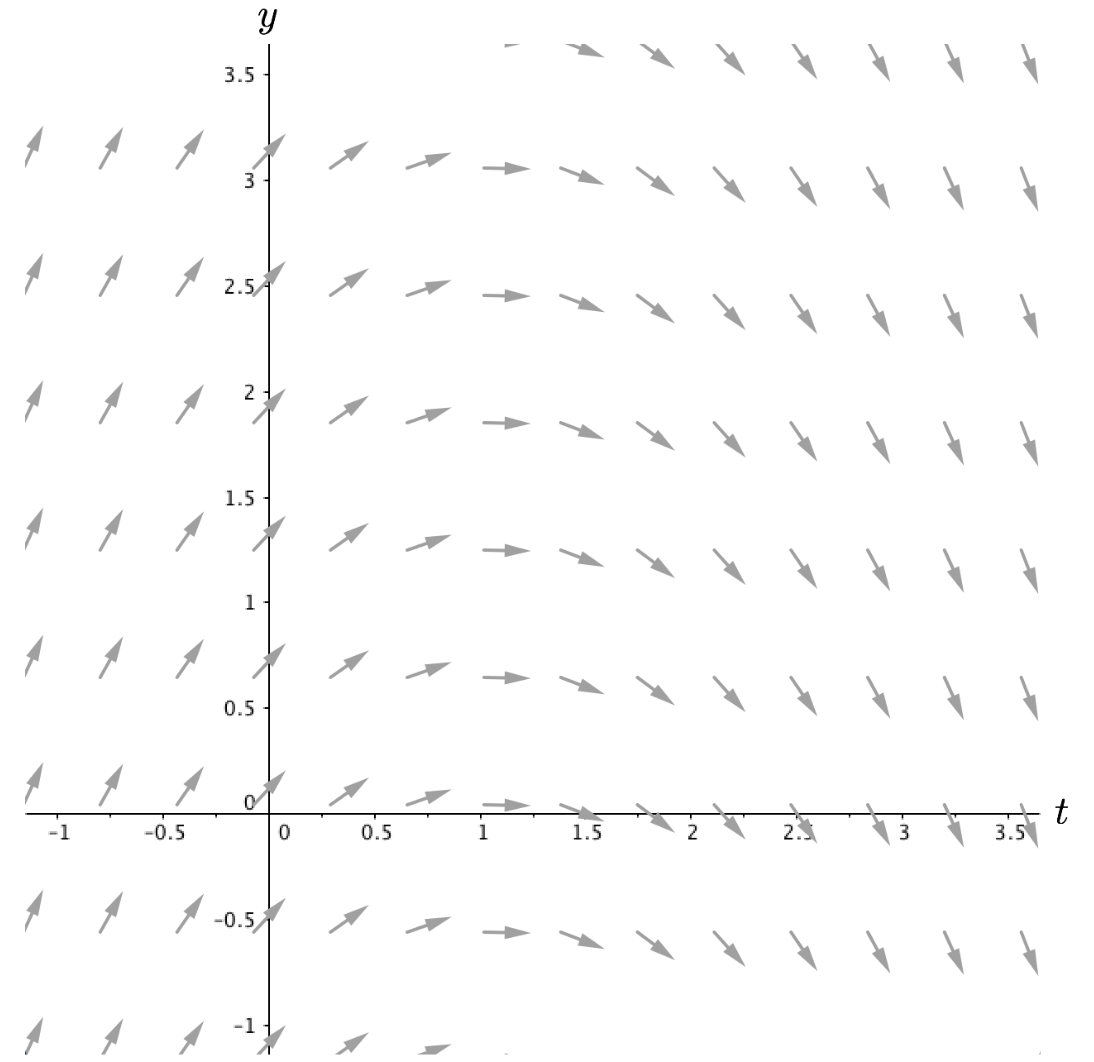
\includegraphics[width=2.75in]{02/02SlopeField3.png} \label{01problem8partc}
\end{enumerate*}
\vspace{0.1in}
\item For each of the slope fields in the previous problem, sketch in graphs of several different qualitatively correct solutions. \label{01problem9}
\vfill

\end{enumerate}


\end{document}
%%%%%%%%%%%%%%%

\clearpage

\pagebegin{Homework Set 1}
 
\begin{enumerate}

\item	Consider the following systems of rate of change equations: \label{01HWproblem1}

\begin{center}
\begin{tabular}{cp{1cm}c}
\textbf{System A}	&& \textbf{System B}  \\

$\displaystyle \begin{aligned}[t]
        \frac{dx}{dt} &= 3x\left(1-\frac{x}{10}\right)-20xy\\
        \frac{dy}{dt} &= -5y+\frac{xy}{20}
        \end{aligned}$	&&				
 $  \displaystyle \begin{aligned}[t]
        \frac{dx}{dt} &= 0.3x -\frac{xy}{100}\\
        \frac{dy}{dt} &= 15y\left(1-\frac{y}{17}\right) +25xy
        \end{aligned}$
\end{tabular}	
\end{center}		 

In both of these systems, $x$ and $y$ refer to the number of two different species at time $t$. In particular, in one of these systems the prey are large animals and the predators are small animals, such as piranhas and humans. Thus it takes many predators to eat one prey, but each prey eaten is a tremendous benefit for the predator population. The other system has very large predators and very small prey. \\

Figure out which system is which and explain the reasoning behind your decision. 

\item Consider the rate of change equation  \[ \frac{dy}{dt}=0.5y(2+y)(y-8),\] which has been created to provide predictions about the future population of rabbits over time.  
\begin{enumerate}
\item	For what values of $y$ is $y(t)$ increasing?  Explain your reasoning.
\item	For what values of $y$ is $y(t)$ decreasing?  Explain your reasoning.
\item	For what values of $y$ is $\displaystyle \frac{dy}{dt}$  neither positive nor negative?  What does this imply about the solution function $y(t)$? \label{01HWproblem2}
\end{enumerate}

\item Valeria created the following graph to help her analyze solutions to the differential equation $\displaystyle \frac{dy}{dt} = 2y \left(1-\frac{y}{10} \right)$. What is this a graph of ({\em i.e.}, what are the axes for this graph)? What information about solutions can you glean from this graph? \label{01HWproblem3}
\begin{center}
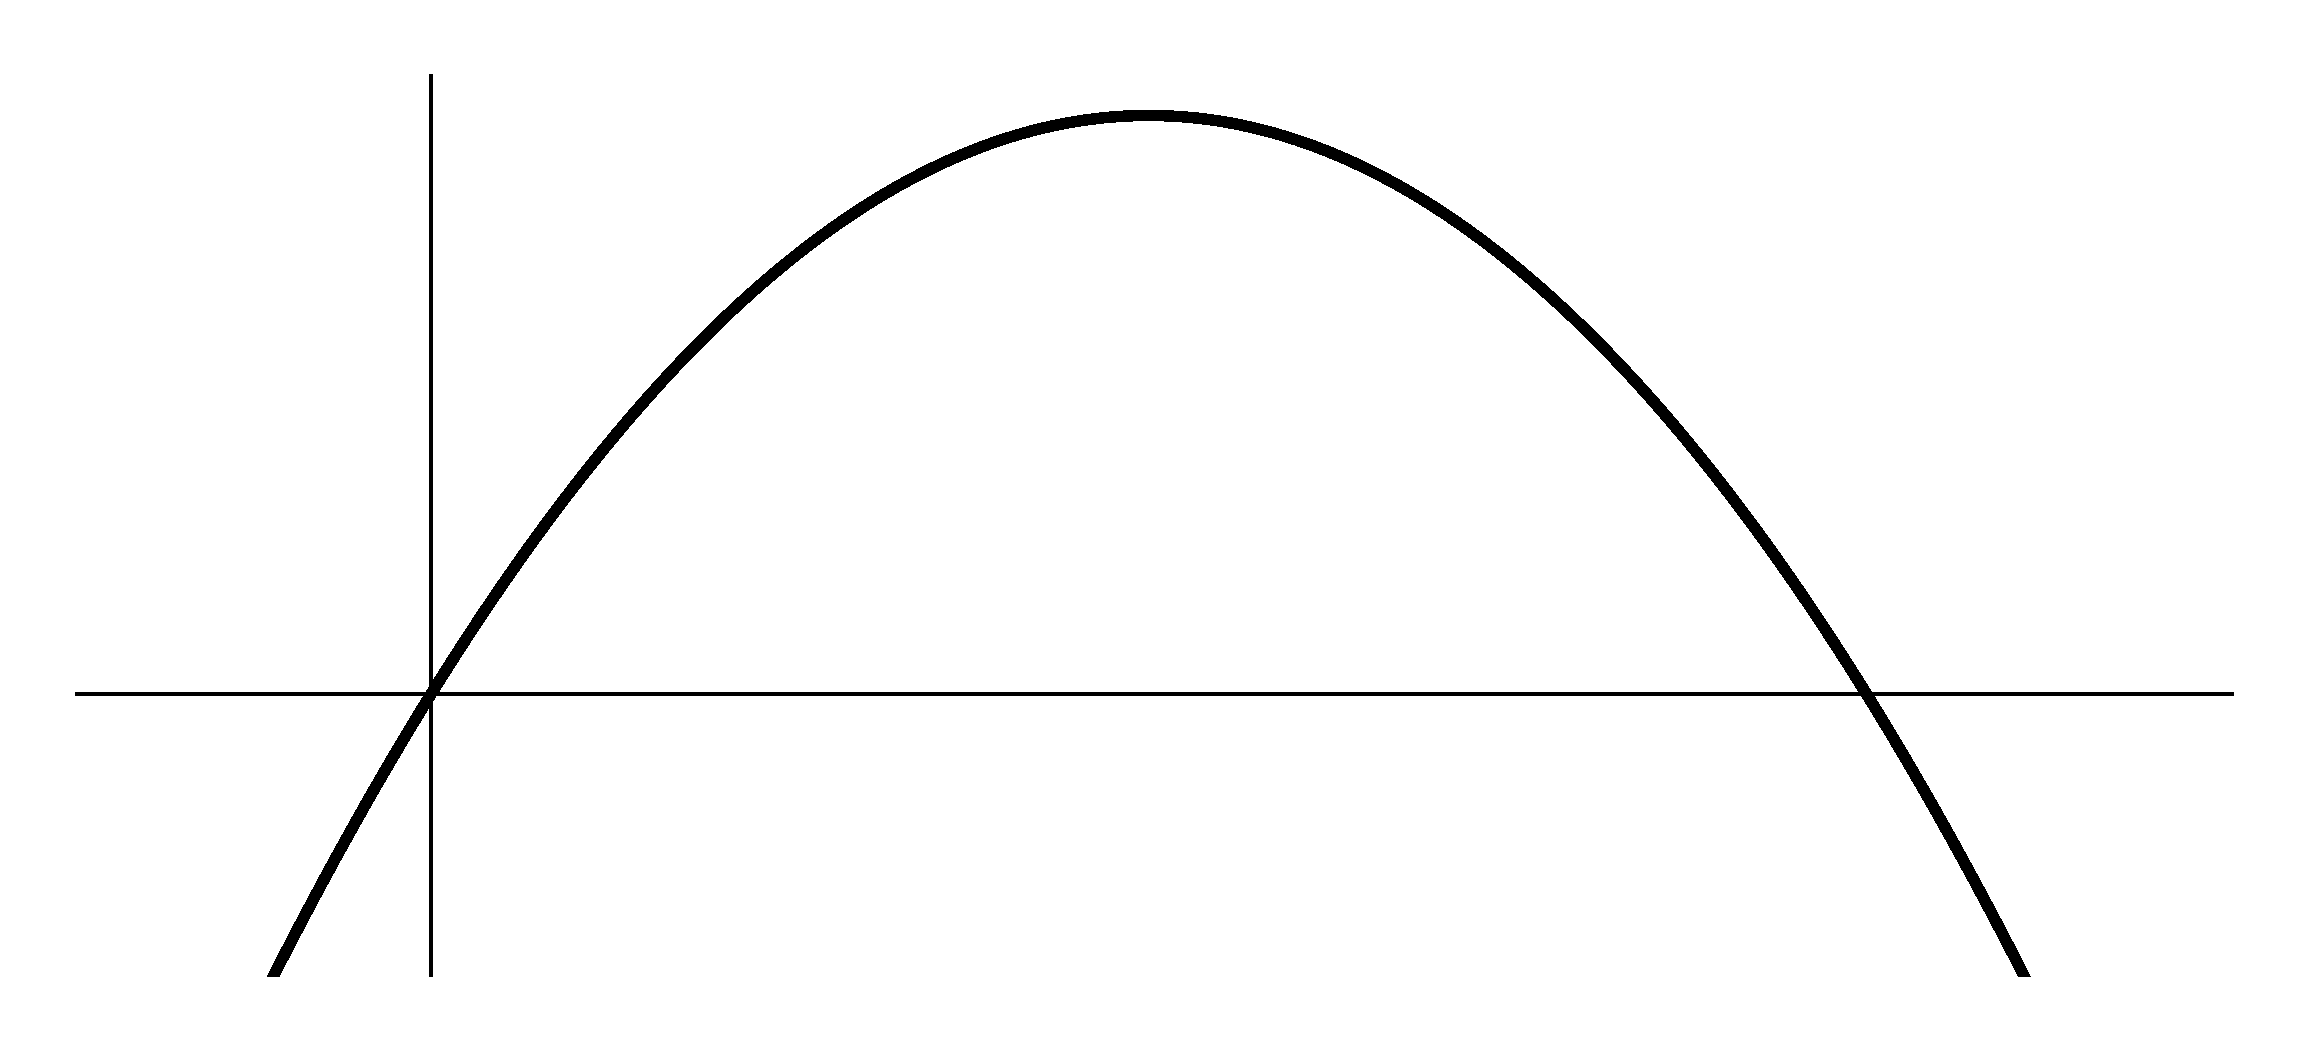
\includegraphics[width=5in]{01/01ValeriaGraph.pdf}
\end{center}

\item  Suppose two students are memorizing the elements on a list according to the rate of change equation \[\frac{dL}{dt}=0.5(1-L),\] where $L$ represents the fraction of the list that is memorized at any time $t$.
\begin{enumerate}
\item	If one of the students knows one-third of the list at time $t = 0$ and the other student knows none of the list, which student is learning most rapidly at this instant? Why?
\item	What does the rate of change equation predict for someone who begins with the list completely memorized? Explain.
\item	Suppose now that the list is infinitely long, like the decimal representation for $\pi$. In reality no one can memorize all the digits to $\pi$, but what does the rate of change equation predict will happen for a person who starts out not knowing any of the digits? That is, according to the rate of change equation, if $L = 0$ at time $t = 0$, is there ever a value of $t$ for which $L = 1$? Explain. 

\end{enumerate}

\item The letter $y$ appears in two places in the differential equation $ \displaystyle \frac{dy}{dt} = 0.3y.$
Is it appropriate to think of both occurrences of $y$ as function of $t$? Explain.


\item In algebra, the goal of solving an equation such as $x^2 + 4x =2$ is to find the values of $x$ that make a true statement. In differential equations, what is the goal of solving an equation such as $\displaystyle\frac{dx}{dt}+4x=2$? 

\item  For the differential equation   $\displaystyle \frac{dy}{dt}=1-y^2$,
\begin{enumerate}
\item	Sketch a slope field by hand. 
\item	Describe any shortcuts or patterns you used to make the task easier.
\item	Sketch several $y(t)$ graphs.
\end{enumerate}

\item Differential equations are often referred to as mathematical models. Explain what the phrase ``mathematical model'' means to you, what previous experiences you have had with mathematical models, and how the mathematical use of the word model is similar to and/or different from the everyday use of the word model ({\em e.g.}, fashion model, model airplane, model student).



\end{enumerate}

